\chapter{Density functional polarisation theory}
\label{chaptertddft}
\section{Time-dependent Density Functional Theory in periodic systems}
Density functional theory (DFT)\cite{PhysRev.140.A1133,PhysRev.136.B864} is a standard approach for calculating ground-state properties of extended and finite systems\cite{doi:10.1021/jp960669l,RevModPhys.87.897}. Time-dependent density functional theory (TDDFT) is an extension of the ground-state formalism that allows to investigate the properties and dynamics of many-body systems in the presence of time-dependent potential. TDDFT is based on the Runge-Gross (RG) theorem\cite{PhysRevLett.52.997}  that establishes a one-to-one correspondence between time-dependent densities and time-dependent one-body potentials. For example when we consider an isolated molecule and an electric filed as  perturbation by means of TDDFT we have access its optical response. As for the DFT case, the RG theorem just guarantees the existence of the mapping, but do not provide a way to construct it. Different approximations for the time-dependent (or frequency dependent) exchange-correlation functional have been proposed in the literature. Exchange correlation functional have been obtained from the ones of the DFT, including long range corrections or derived from more accurate methods\cite{Onida,faber2014excited}. The response equations of TDDFT have been encoded in standard quantum chemical packages\cite{valiev2010nwchem}, and real-time TDDFT is currently used to simulate the short time dynamics of excited electrons\cite{PSSB:PSSB200642067}.\\
Despite the success of TDDFT in molecular systems, the situation is more complicated in extended system. 
In fact, although other methods, as for instance Green's function theory\cite{strinati}, provide a similar accuracy in extended\cite{Aulbur19991} and finite systems\cite{blase2011charge,faber2012electron}, this is not the case of TDDFT.\\
Due to the lower computational cost of TDDFT respect to Green's function formalism it would be desirable to have the same accuracy in extended and finite systems.\\
The first idea one can have it is that the available exchange correlation functionals, for some reason, are not enough precise to describe excitation in solids. Unfortunately the problem is more serious.\cite{maitra2003current}
In order to understand from where the problem originates, let's go back to the original statement of the RG theorem.
In the first part of the proof, RG established a one-to-one correspondence between potentials and currents.  Then in the second part of their work, they used the continuity equation to relate currents to densities in order to prove the mapping between densities and potentials.  The problem in the RG proof stays in the use of the continuity equation. As we saw in the introduction to chapter~\ref{chapterberry} there is not a univoque mapping between current and density in periodic systems. 
In fact the mapping between currents and densities requires that certain surface integral involving the density and the potential vanishes. For finite systems this condition  can be given rigorously at the surface in which the density vanishes. For a periodic system, one might try to choose a surface around which the density and potential are periodic but for a uniform field the linearity of the potential prevents this, and TDDFT does not apply. \\
The problem of TDDFT in periodic system was also illustrated  by means of a simple example in the paper of Maitra et. al.\cite{maitra2003current}. They considered a free electron gas on a ring subjected to a constant uniform electric field. In this case it is possible to write down the exact solution of the problem. One finds that the electric field modifies only the phase of the single particle orbitals, leaving the density unchanged. This result shows that different electric fields  give rise to exactly the same density and therefore there is not an unique mapping between density and external field.\\
In order to solve the problems with TDDFT in periodic systems and extension was presented some years ago, the Time-Dependent Current Density Functional Theory(TDCDFT)\cite{PhysRevA.38.1149}. This formulation uses the direct mapping between the external potential and the current density, without reels on the continuity equation.\\
In this section we will use a simplified versions of TDCDFT, i.e. the Density-Functional Polarization Theory (DFTP).  In DFTP one uses the relation between polarization and current to construct a theory that relies on density and polarization instead of current density. The possibility to use the polarisation as additional variable besides the density it is a valid approximation when it is possible to disregard the transverse term of the current. Since we are interested in the optical response in the limit of long-wave length limit, this is a valid approximation.\\
In the rest of this chapter we will introduce DFTP, and explain how to build functionals in term of polarization and density. Then we will use these functionals in our real-time approach to study non-linear response of bulk semiconductors.
\section{General Introduction}
%Time-dependent density-functional theory\cite{PhysRevLett.52.997} (TD-DFT) is a standard tool in the computation of the optical response of molecules and in general of finite systems. In contrast TD-DFT is rarely employed for the study of the optical response of extended systems such as periodic crystals. The main reason is that within the common approximations TD-DFT fails to describe excitonic effects which typically dominate the optical spectra of insulators and semiconductors.~\cite{botti2007time} 
%Though commonly attributed to the approximation for the exchange-correlation density functional, the problem of TD-DFT for periodic crystals is more fundamental. Calculations of optical response of periodic crystal use periodic boundary conditions. TD-DFT is based on the Runge-Gross theorem~\cite{PhysRevLett.52.997} that establishes the one-to-one correspondence between the time-dependent densities and scalar external potentials. 
In periodic systems in presence of a time-dependent homogeneous electric field only the one-to-one correspondence between the time-dependent currents and potentials (scalar and vector) can be established and time-dependent current density functional theory (TD-CDFT) is then the correct theoretical framework.~\cite{maitra2003current,PhysRevA.38.1149} In particular it is the optical limit, i.e. the case in which the transferred momentum $\qq\ra 0$,  which cannot be described starting from the density only. 
One could still work with functionals that depends on the density--only, but there is a price to pay. All the equations have to be worked out with a finite but very small momentum  and the $\qq\ra 0$ limit can be performed only at the end of the calculation. 
Furthermore in order to describe excitonic effect the exchange--correlation functionals have to be ultra--nonlocal and to diverge as $\qq \ra 0$.~\cite{PhysRevLett.88.066404} Such an approach is used within the linear response framework but it is not feasible within a real time framework since for practical reasons calculations have to be performed directly at $\qq=0$. Thus one needs to go beyond the density--only treatment. As a clear indication of this, the macroscopic polarisation and the response functions cannot be calculated within a density--only scheme at $\qq=0$.~\cite{PhysRevB.9.1998}
Problems are not limited to the time--dependent case. Even in the static limit, e.g. for dielectrics in a static homogeneous electric field, Gonze and coworkers proved that {\em ``the potential is not a unique functional of the density, but depends also on the macroscopic polarisation''}.~\cite{Gonze1995} In this case then the theory has to be generalised to consider functionals of both the density and the polarisation in what is called density--polarisation functional theory (DPFT). The latter can be obtained from TD-CDFT in the static limit.

Here we propose a real--time approach based on DPFT for calculating the optical response properties of dielectrics, thus considering functionals of both the time--dependent density and the macroscopic bulk polarisation.
Real--time approaches allows in principle to calculate the optical response at all order so to access nonlinear properties\cite{takimoto:154114}, including nonperturbative extreme nonlinear phenomena\cite{lee2014first} and to simulate real--time spectroscopy experiments.\cite{otobe2015femtosecond} It is highly desirable then to have computational inexpensive first principles real--time approaches, such as TD-DFT, that include excitonic effects.            
In particular here we consider an effective electric field which is a functional of the macroscopic polarisation. We employ simple local functionals of the polarisation~\cite{maitra2003current,PhysRevLett.115.137402} either fitted to reproduce the linear optical spectra\cite{LRC} or derived from the jellium with gap model kernel.~\cite{jgm}

In the following, we review DPFT and we extend it to the case of time-dependent electric fields. We discuss briefly the approximations for the effective-electric field and we present how the relevant response functions are calculated from the macroscopic polarisation.  Then, we show that for the optical absorption, the second- and third-harmonic generation of semiconductors  the simple local functionals of the polarisation account for excitonic effects similarly to the ultranonlocal kernel within the density-only response framework. In the conclusion we discuss the proposed approach as an alternative to existing schemes based on TD-DFT and TD-CDFT. 



%********************************************************
\section{Density polarisation functional theory}
%********************************************************

%The coupling of an external electromagnetic field with a dielectric is described via the electromagnetic potentials and thus is gauge dependent.
%In the present manuscript we use the length gauge which is obtained from the multipolar gauge within the electric-dipole approximation (EDA).~\cite{Kobe1982}. 
%This implies that we assume a spatially uniform electric field. Such macroscopic electric field enters via a scalar potential,
%$\varphi(\rr)=-\Efield^{\text{ext}} \cdot \rr$, whose corresponding energy has generally the form
%\be
%E_\varphi= -\Omega\, \Efield^{\text{ext}} \cdot \PP 
%\label{eq:enphi}
%\ee
%where $\Omega$ is the volume and $\PP$ is the bulk macroscopic polarisation that is then the key quantity to describe the coupling of dielectrics with external fields 
%(in the velocity gauge the coupling would have been instead via the macroscopic current). 
%
%For finite systems (i.e. in which the electronic density $n$ goes to zero when $\rr\rightarrow \infty$), Eq.~\ref{eq:enphi} is equivalent to 
%$\int n(\rr) \varphi(\rr) d\rr$ and $\PP = \int n(\rr) \rr d\rr$.  
%However these expressions are ill-defined when periodic boundary conditions are imposed.~\cite{Blount} The Modern Theory of Polarization~\cite{RevModPhys.66.899} provides a correct definition for the macroscopic bulk polarisation in terms of the many-body geometric phase.
%For a system of independent particles in a periodic potential the polarisation ${\cal \PP}$ along the Cartesian direction $\alpha$ is given by~\cite{KSV1} 
%\be
%{\cal P}_\alpha = -\frac{ief}{(2 \pi)^3} \sum_{n}^{\text{occ}} \int d\kk \langle  u_{\kk n} |\partial_{k_\alpha}  u_{\kk n} \rangle, \label{berryP3} 
%\ee
%where $f$ the spin occupation, and $|u_{\kk n}\rangle$ the periodic part of the Bloch function $|\phi_{\kk n}\rangle$.  
%
%Equation~(\ref{berryP3}) seems to suggest that, though $\PP$ cannot be expressed as an explicit functional of the electron density $n$, it is still an implicit functional of $n$ through the Bloch functions obtained from the solution of the KS equation. As we discuss in the following subsection however, for a dielectric in a macroscopic electric field the macroscopic polarisation needs to be considered as an independent variable. Accordingly
%the macroscopic part of the external electric field $\Efield^{\text{ext}}$ cannot be included via the potential $v^{\text{ext}}$,
%since the associated energy functional would be ill-defined.
%In such approach the KS equations and the associated Bloch functions depend on both the density and the macroscopic
%polarisation of the system.

\subsection{Static case}
%********************************************************
An infinite periodic crystal (IPC) in a macroscopic electric field $\Efield^{\text{ext}}$ does not have a ground-state. Therefore the Hohenberg-Kohn theorem cannot be applied and DFT cannot be used. In particular the density does not suffice to describe the system as the one-to-one mapping between density and external potential does not hold: one can devise an external macroscopic electric field that applied to a system of electrons in an IPC does not change its density $n$.
The works of Gonze Ghosez and Godby,~\cite{Gonze1995} Resta~\cite{Resta1996}, Vanderbilt~\cite{Vanderbilt1997} and of Martin and Ortiz~\cite{Martin1997} established that in addition to the density, the macroscopic (bulk) polarisation $\PP$ is needed to characterise IPC in a macroscopic electric field. With some cautions the proof of the Hohenberg-Kohn theorem can be extended~\cite{Martin1997} to demonstrate the existence of the invertible mapping
$$(n(\rr),\PP)\leftrightarrow (\bar v^{\text{ext}}(\rr),\Efield^{\text{ext}}) $$
where $ \bar v_{\text{ext}}$ is the periodic microscopic part of the external potential.
Then the total energy of an IPC is a functional of both the electron density $n$ and the macroscopic polarisation $\PP$:
\be \label{eq:dpften}
E[n,\PP] = \bar F[n,\PP]+ \int_\Omega n(\rr) \bar v^{\text{ext}}(\rr)\,d\rr  -\Omega\, \Efield^{\text{ext}} \cdot \PP,
\ee 
where $\bar F$, the internal energy, is a universal functional of both $n$ and $\PP$ (see Ref.~\cite{Martin1997} for details),
and is defined in the usual way
as the sum of the expectation the kinetic and electron-electron interaction operators
\be
\bar F[n,\PP] = \langle \Psi | \hat T + \hat V_{ee} |\Psi \rangle.
\ee 
The difference with the internal energy within standard DFT is that the $N$-particle wavefunction $\Psi$ is not an eigenstate of the original Hamiltonian (which does not have a ground state), but of an auxiliary Hamiltonian which commutes with the translation operator (see Ref.~\cite{Martin1997} for details). Notice that DPFT is not the only way to treat IPC in a electric field within a density functional framework: as an alternative Umari and Pasquarello proposed $\Efield$-DFT, a density functional theory depending on the electric field.~\cite{Umari2005}   

The Kohn-Sham equations can be extended as well to treat IPC in a macroscopic electric field.~\cite{Martin1997}
In particular the Kohn-Sham crystal Hamiltonian takes the form:%compare with Souza expressions 
\be \label{eq:dpftks}
H^{s}_\kk
= -\frac{1}{2}\left(\nabla + i\kk\right )^2 + \bar v^{s}(\rr) -\Omega\Efield^{s}\cdot \nabla_\kk %CHECK
\ee
which is a functional of both the density and the polarisation.
In Eq.~\eqref{eq:dpftks}  the Kohn-Sham microscopic (periodic) potential $\bar v^{s}$ is defined as
\be\label{eq:kspot}
\bar v^{s}(\rr) = \bar v^{\text{ext}}(\rr) +  \bar v^{\text{H}}(\rr) + \bar v^{\text{xc}}(\rr) 
\ee
$\bar v^{\text{ext}}(\rr)$, $\bar v^{\text{H}}$ are respectively the microscopic external and Hartree potential.
The total classical potential is defined as $\bar v^{\text{tot}}(\rr)=\bar v^{\text{ext}}(\rr)+\bar v^{\text{H}}(\rr)$.
$\bar v^{xc}$ is the functional derivative of the exchange--correlation energy with respect to the density.
$\bar v^{\text{ext}}(\rr)$ here describes the field generated by the ions, i.e. the electron--ion interaction
in the Coulomb gauge and neglecting retardation effects.
The last term of the RHS of Eq.~\eqref{eq:dpftks}---that originates from the last term in the RHS of Eq.~\eqref{eq:dpften}---constitutes
the key difference with respect to the zero-field KS equations.
$\nabla_\kk$~is the polarisation operator derived by functional-differentiating
$\PP$ [Eq.~\eqref{berryP2}] with respect to the KS eigenstates.
$\Efield^{s}$ is the KS macroscopic field  
\be
%\Efield^{ks} = \Efield^{\text{tot}} + \Efield^{\text{xc}}
\Efield^{s} = \Efield^{\text{ext}} + \Efield^{\text{H}}  + \Efield^{\text{xc}},
\label{eq:ksfld}
\ee
that contains the corresponding macroscopic components of $\bar v_s$. Note that these macroscopic components cannot be included via the potential which would be ill defined when imposing periodic boundary conditions.  
The $\Efield^{\text{xc}}$ is defined as the partial derivative of the xc energy with respect to the polarisation density field.
The sum of the macroscopic external and Hartree fields defines the total classical field:
\be
\Efield^{\text{tot}} = \Efield^{\text{ext}} + \Efield^{\text{H}}. 
\label{eq:totfld}
\ee    

At zero-field, that is when no macroscopic external electric field $\Efield^{\text{ext}}$ is applied,
the macroscopic component of the ionic potential and of the Hartree component exactly cancel as a consequence of the charge neutrality of the system and  
the macroscopic xc component vanishes.
In this situation  standard density-only functional theory can be used. 



As $\bar v^{s}$ and $\Efield^{s}$ are functionals of the density and the polarisation, the Kohn-Sham equations
for the KS orbitals $\{\phi_{n\kk}\}$  have to be solved self-consistently with the density (spin unpolarized case)
\be
n(\rr) = 2 \sum^{\text{occ}} |\phi_{n\kk}(\rr)|^2 
\ee
and the polarisation expressed in terms of a Berry phase [Eq.~\eqref{berryP2}].


\subsection{Time-dependent case}
The Runge-Gross theorem \cite{PhysRevLett.52.997} is the basis of TD-DFT. It establishes the one-to-one mapping between the time-dependent scalar potential and the time-dependent density. For the case in which a time-dependent vector potential is present Ghosh and Dhara~\cite{PhysRevA.38.1149} showed that the mapping can be established between the current-density and the vector potential. More recently Maitra and co-workers~\cite{maitra2003current} showed that TD-CDFT is the correct framework for IPC in homogeneous electric fields.

The time-dependent change in the polarisation density field $\pp$ is related to the time-dependent current-density $\jj$ by 
\be
\pp (\rr;t) = \int^t_{-\infty} dt' \jj(\rr;t') 
\ee
In a dielectric we can then use either $\pp(\rr,t)$ or $\jj(\rr, t)$ as main variable to describe an IPC in a time-dependent finite homogeneous electric field. Furthermore we can consider separately the microscopic and the macroscopic components of $\pp(\rr, t)$: $\PP (t)$ and $\bar \pp(\rr, t)$. The latter quantity is fully determined by the density through the continuity equation.
Then we can extend to the time-dependent case the one-to-one mapping
$$(n(\rr,t),\PP(t))\leftrightarrow (\bar v^{\text{ext}}(\rr,t),\Efield^{\text{ext}}(t)). $$
The time--dependent Kohn-Sham crystal Hamiltonian has the same form of the equilibrium KS Hamiltonian [Eq.~\eqref{eq:dpftks}] with the only difference that now potentials and wavefunctions are time--dependent:
\be \label{eq:tdksh}
H^{s}_\kk(t)
= -\frac{1}{2}\left(\nabla + i\kk\right )^2 +  \bar v^{s}(\rr,t) -\Omega\, \Efield^{s}(t)\cdot \nabla_\kk
.
\ee
We rewrite the external field and potential as the contribution at equilibrium, $\Efield^{\text{ext},0}$ and $\bar v^{\text{ext},0}(\rr)$  plus the time-dependent perturbation:
\bea
\Efield^{\text{ext}}(t)&=&\Efield^{\text{ext},0}+\Delta \Efield^{\text{ext}}(t), \\
\bar v^{\text{ext}}(\rr,t)&=&\bar v^{\text{ext},0}(\rr) +\Delta v^{\text{ext}}(\rr,t) .
\eea  
Then,
\bea
\bar v^{s}(\rr,t) &=& v^{s,0}(\rr) +\Delta  \bar v^{s}(\rr,t) \\
\Efield^{s}(t)     &=&\Efield^{s,0}+\Delta \Efield^{s}(t),
\eea
where the $0$ superscript denotes that the functional is evaluated 
in presence of the equilibrium fields, thus at equilibrium density and polarisation.  We then restrict ourselves to consider  the case with no external macroscopic electric field at equilibrium, i.e. ${\Efield^{\text{ext},0}=\mathbf{0}}$, and to a macroscopic-only time dependent perturbation, i.e. $\Delta \bar v^{\text{ext}}(\rr,t)=0$.
Therefore
\bea
\Delta \bar v^{s}(\rr, t ) &=& \Delta\bar v^\text{H}+\Delta\bar v^{\text{xc}} \\
\Delta\Efield^{s}(t)&=&\Efield^{s}(t)
\eea
Finally, the TD-KS equations for the periodic part $u_{n\kk}$ of the Bloch function 
can be expressed as
\be
  i\partial_t u_{n\kk} =\left( H^{s,0}_\kk +  \Delta \bar  v^{s}(\rr,t) -\Omega\, \Efield^{s}(t)\cdot \nabla_\kk \right)u_{n\kk}
,
\label{eq:kseom}
\ee
and have to be solved consistently with the time-dependent density and polarisation.
The latter has the same form of the static polarisation [Eq.~\eqref{xtrace}] with
the difference that $|v_{\kk n}\rangle$ are the time-dependent valence bands.

In the time dependent case and within the EDA,
it can be shown straightforwardly that the Hamiltonian
in Eq.~\eqref{eq:tdksh} can be derived from the KS Hamiltonian of TD-CDFT
with a gauge transformation from the velocity to the length gauge.\cite{maitra2003current}


%*****************************************************************
\section{Expressions for the Kohn-Sham electric field}
\label{sc:ksef}
%*****************************************************************

The KS electric field in Eq.~\eqref{eq:ksfld} is the sum of three components. It seems natural to consider the external component $\Efield^{\text{ext}}$ as an input of the calculation, i.e. $\Efield^{\text{ext}} = \Efield^{\text{inp}}$. The total classical field $\Efield^{\text tot}$ is then calculated from Eq.~\eqref{eq:totfld} by adding the Hartree component that in the EDA is the polarisation $\Efield^{H} = 4 \pi \PP$. This is not the only possible choice nor always the most convenient. When calculating linear and nonlinear optical susceptibilities, which do not depend on the total or external fields, it is numerically more convenient to choose the total classical field as input field. As this work objective is the calculations of optical susceptibilities we adopt indeed $\Efield^{\text{inp}} = \Efield^{\text{tot}}$.  The two choices for the input field, i.e. either the total or external field, have been referred as ``longitudinal geometry'' and ``transverse geometry'' by Yabana and coworkers\cite{PhysRevB.85.045134} and are discussed in more length in Appendix~\ref{appA}. 

While the choice of the input field is a matter of computational convenience, the choice of the expression for the xc macroscopic electric field is critical to the accuracy of the results. Like the microscopic xc potential no exact expression is known and one should resort to an approximation for the functional form of the xc field. Contrary to the microscopic xc potential for which hundreds of approximations exist,\cite{libxc} except for the work of Aulbur and coworkers~\cite{aulbur1996polarization} we are not aware of approximations for the xc macroscopic field. What does exist in the literature are xc kernels within the TD-DFT and TD-CDFT that give a non-zero contribution to the response in the optical limit. In what follows we link the xc kernel with the macroscopic field (similarly to Refs.~\cite{maitra2003current,PhysRevLett.115.137402}). 
In fact in the linear response limit the exchange-correlation electric field is related to the polarisation $\pp$ (see for example Refs.~\cite{maitra2003current},~\cite{PhysRevLett.115.137402})
through the xc kernel $\newtensor{F}^{\text{xc}}_{}$. The latter describes how the xc electric field (both microscopic and macroscopic) changes when the polarisation is perturbed. $\newtensor{F}^{\text{xc}}_{}$ can be defined independently through the Dyson equation connecting 
the polarisation response function of the physical system, $\newtensor{\chi}$,
to the polarisation response function of the KS system, $\newtensor{\chi^s}$. 
By rewriting the relation between $\Efield^{\text{xc}}$ and $\newtensor{F}^{\text{xc}}_{}$ in reciprocal space~\footnote{In general the expression of the xc electric field in terms of $\tensor{F}^{\sss XC}_{}$ is an integral along a path in the infinite dimensional space of the densities/macroscopic polarizations. Such integral does not depend on the path if $\tensor{F}^{\sss XC}_{}$ is defined as a functional derivative of some function. Furthermore here we consider the case where $\tensor{F}^{\sss XC}_{}$ is a local (or semi--local) functional. Then the infinite dimensional integral reduces to a simple three-dimensional integral which, in reciprocal space, can be represented as a sum over the $\GG$ vectors.} one obtains~\cite{maitra2003current} for the macroscopic component ($\GG=0$) 
\begin{multline}
\Efield^{\text{xc}}(t)= \int dt' \Big[ \newtensor{F}^{\text{xc}}_{\sss 00}(t-t') \PP(t')  \\
               -{i} \sum_{\GG' \neq 0} \newtensor{F}^{\text{xc}}_{\sss 0\GG'}(t-t')\frac{ n_{\sss \GG'}(t')}{{\rm G'}^2}\GG' \Big] 
\label{Excmac}
\text{,}
\end{multline}
and for the microscopic components $\efield^{\text{xc}}_{\sss \GG}$ ($\GG\neq 0$)
\begin{multline}
\efield^{\text{xc}}_{\sss \GG}(t)= \int dt' \Big[ \newtensor{F}^{\text{xc}}_{\sss \GG 0}(t-t') \PP(t')  \\
                    -{i} \sum_{\GG' \neq 0} \newtensor{F}^{\text{xc}}_{\sss \GG\GG'}(t-t')\frac{ n_{\sss \GG'}(t')}{{\rm G'}^2}\GG' \Big] 
\label{Excmic}
\text{.}
\end{multline}
The first term on the RHS of Eq.~\eqref{Excmac} is directly proportional to the macroscopic polarisation, the second term involves the density and is the microscopic contribution to the macroscopic field. Note that as we assume the EDA we do not have the contribution from the microscopic transverse current as in Maitra and coworkers.~\cite{maitra2003current}
The variation of the microscopic xc potential $\Delta \bar v^{\text{xc}}$ can be written in terms of the microscopic components $\efield^{\text{xc}}_{\sss \GG}$ as
\be
\Delta \bar v^{\text{xc}}_{\sss \GG}(t) =  i \frac{\GG \cdot  \efield^{\text{xc}}_{\sss \GG}(t) }{{\rm G}^2}.
\label{eq:pot_from_exc}
\ee
  
Berger~\cite{PhysRevLett.115.137402} has recently proposed an approximation for $\newtensor{F}^{\text{xc}}_{00}$ from current-density functional theory. The approximation however requires the knowledge of the Random-Phase-approximation (RPA) static dielectric function: while within a linear response approach this does not require any additional calculation, within a real-time approach the RPA static dielectric function needs to be computed beforehand. Furthermore Berger~\cite{PhysRevLett.115.137402} neglects the microscopic contribution.

An alternative way to derive approximations for $\newtensor{F}^{\text{xc}}_{}$ is to rely on the standard TD-DFT xc kernel $f^{\text{xc}}_{}$. The latter describes how the xc potential changes when the density is perturbed and is defined from the Dyson equation relating the density-density response of the physical and the KS system. The two kernels can be related via the equation
\be 
f^{\text{xc}}_{\sss \GG \GG'}(\qq\rightarrow 0; t - t') = \lim_{\qq\rightarrow 0} \frac{\newtensor{F}^{\text{xc}}_{\sss \GG \GG'}(t-t') \cdot \newtensor{g}}{|\qq + \GG||\qq + \GG'|}.  
\label{eq:k2k}
\ee 
where $\newtensor{g}$ is the metric tensor.

For example the long-range corrected (LRC) approximations $f^{\text{xc}}\approx f^{\sss LRC}$, which take the form
\be
f^{\sss LRC}_{\sss \GG\GG'}(\qq\rightarrow 0; t-t') =
  \lim_{\qq\rightarrow 0} \frac{-\alpha^{\sss LRC}\delta_{\sss \GG,\zero}\delta_{\sss \GG',\zero}}{|\qq|^2}\delta(t-t'),   
\label{jgmqzero}
\ee
can be used. Then $\newtensor{F}^{\text{xc}}_{\sss \zero\zero} \cdot \newtensor{g}$ can be approximated with any of the $\alpha^{\sss LRC}$ (we assume $\alpha > 0$) proposed in the literature. Unfortunately all the approximations proposed so far~\cite{LRC,PhysRevB.72.125203} neglect the dependence of $\alpha$ on the reciprocal lattice versors. Furthermore most of the approximations relies on empirical parameters, with the exception of the family of bootstrap kernels~\cite{PhysRevLett.114.146402,PhysRevLett.107.186401} that relate $\alpha$ to the electronic screening in an expression equivalent to that derived by Berger from TD-CDFT.

In this work, we derive the $\newtensor{F}^{\text{xc}}$ needed in Eq.~\eqref{Excmac} from the Jellium with Gap Model (JGM) kernel proposed by Trevisanutto and coworkers.\cite{jgm}
The latter kernel is a functional of the electronic density $n$ and of the fundamental gap of the material $E_{\text{gap}}$. In the optical limit the JGM kernel takes the form of a long-range corrected approximation
with $\alpha^{\sss LRC}$ defined as the cell average~\cite{jgm} of
\be
\alpha^{\sss JGM}(\rr;t) = 4\pi \tilde B \left[1 - \exp{\left( -\frac{E_{\text{gap}}^2}{4\pi n \tilde B} \right)} \right].  
\label{eq:alpha}
\ee
In the equation above $\tilde B = (B + E_{\text{gap}})/(1 + E_{\text{gap}})$, where $B=B[n]$ is a functional of the density found by fitting the local field factor of the homogeneous electron gas from Quantum Montecarlo data.~\cite{PhysRevB.57.14569}   
 
For cubic systems we thus consider $\newtensor{F}^{\text{xc}}\approx\newtensor{F}^{\sss JGM}$ with
\begin{subequations}
\begin{gather}
\newtensor{F}^{\sss JGM}_{\sss \zero\GG}(t-t') = -\frac{1}{2}\alpha^{\sss JGM}_{\sss \GG}(t) \newtensor I \delta(t-t') \\
\newtensor{F}^{\sss JGM}_{\sss \GG\zero}(t-t') = -\frac{1}{2}\alpha^{*\sss JGM}_{\sss \GG}(t) \newtensor I \delta(t-t').
\end{gather}
\label{eq:krnl}
\end{subequations}
where $\alpha^{\sss JGM}_{\sss \GG}(t)$ is the Fourier transform of Eq.~\eqref{eq:alpha} and $\newtensor I$ is the identity tensor. 
Notice that we symmetrized ${F}^{\sss JGM}_{\sss \GG,\GG'}$ so to obtain a Hermitian kernel. Other strategies of symmetrization have been proposed in the literature, see Ref.~\cite{jgm} and reference therein.
Like standard approximations for the kernel this approximation neglects memory effects (i.e. the macroscopic field at time $t$ depends on the values of the density and polarisation only at time $t$) and it is thus frequency independent.

Finally, inserting this approximation for the kernel [Eq.~\eqref{eq:krnl}] in the expression for the xc fields [Eq.~\eqref{Excmac}--\eqref{Excmic}] and using Eq.~\eqref{eq:pot_from_exc} we obtain 
\bea
\Efield^{\sss JGM}(t)&=&\alpha^{\sss JGM}_{\zero}(t)
{\cal \PP}(t)
-\frac{i}{2}\sum_{\sss \GG \neq 0} \alpha^{\sss JGM}_{\sss \GG} (t)\frac{ n_\GG(t)}
{{\rm G}^2}\GG \nonumber \\
\Delta \bar v^{\sss JGM}_{\sss \GG}(t)&=&\frac{i}{2}\sum_{\sss \GG \neq 0}  \frac{\alpha^{*\sss JGM}_{\sss \GG} (t)}{G^2} \GG \cdot {\cal \PP}(t), 
\label{eq:Excapp}
\eea
where the second term in the RHS of Eq.~\eqref{Excmic} is zero due to our symmetrization strategy [Eq.~\eqref{eq:krnl}]. In our calculations we will use either Eq.~\eqref{eq:Excapp} and or an $\alpha^{\text{opt}} \PP$ approximation for the macroscopic xc electric field in which $\alpha^{\text{opt}}$ is a parameter which gives the best agreement between the computed and experimental optical absorption spectra. The two approximations will be referred as JGM polarisation function (JGM-PF) and optimal polarisation functional (opt-PF).

%*****************************************************************
\section{Computational details}
%*****************************************************************

The eigensolutions $\{|\phi^0_{m\kk}\rangle \}$ of the zero-field Hamiltonian are calculated using the plane-wave pseudopotential density-functional code {\sc abinit}~\cite{abinit} within the local density approximation for the exchange-correlation energy. All the numerical details regarding the atomic structure, the number of bands, cutoff and  pseudopotential are detailed in Ref.\cite{gruningtddf1}. 
%We have employed norm-conserving pseudopotentials of the Troullier-Martins type~\cite{troullier} for Si, AlAs and CdTe, and of the Hamann type~\cite{PhysRevB.40.2980} for GaAs. For all the systems we have used four shifted $8 \times 8 \times 8$ Monkhorst-Pack meshes\cite{PhysRevB.13.5188} to converge the ground-state density.   
%The periodic part $\{|u^0_{m\kk}\rangle\}$  of the so-generated eigensolutions are used as a basis to expand the time-dependent KS Bloch-functions (or more precisely their periodic part)
%\be
%|u_{n\kk}(t) \rangle = \sum_m |u^0_{m\kk} \rangle \langle u^0_{m\kk}|u_{n\kk} (t) \rangle =  \sum_m  |u^0_{m\kk} \rangle c^{\kk}_{mn}(t)
%\label{eq:basis}
%\ee
%and the TD-KS equations [Eq.~\eqref{eq:kseom}] can be rewritten as the equation of motions for the coefficients $c^{\kk}_{nm}$. We obtained converged spectra by truncating the sum in Eq.~\eqref{eq:basis} at $m=9$ bands for Si, $m=11$ bands for AlAs and GaAs, and $m=13$ for CdTe. 
%
%\begin{table}[H]
%\begin{tabular}{l|c|c|l|l}\hline\hline
%  System & $K$ (Ha)& $a_{\text{latt}}$ (Bohr) & atom$_1$ & atom$_2$\\
%  \hline
%  Si  &  14 &  10.260 & Si: $\ 3s^23p^2$  &\\
%  GaAs&  30 &  10.677 & Ga: $4s^24p^1$    & As: $4s^24p^3$\\
%  AlAs&  20 &  10.696 & Al: $\ 3s^23p^1$  & As: $4s^24p^3$\\
%  CdTe&  40 &  12.249 & Cd: $4d^{10}5s^2$ & Te: $4d^{10}5s^25p^4$\\
%  \hline\hline
%\end{tabular}
%\caption{\footnotesize{Parameters for the DFT calculations.
%The kinetic energy cutoff $K$,
%the lattice constant $a_{\text{latt}}$ and
%the non frozen electrons explicitly included in valence.}} \label{tb:pardft}
%\end{table}
%
%The derivatives with respect to the crystal momentum that appear in Eqs.~\eqref{berryP2}  and~\eqref{eq:dpftks} for the polarisation and the polarisation operator are evaluated numerically. Following Souza and coworkers~\cite{souza_prb} the polarisation is rewritten as
%\be
%{\cal P}_\alpha = -\frac{ef}{2 \pi \Omega} \frac{\mathbf a_\alpha}{N_{\kk_\alpha^\perp}} \sum_{\kk_\alpha^\perp} \mbox{Im ln} \prod_{i=1}^{N_{\kk_\alpha}-1}\ \mbox{det } S(\kk_i , \kk_i + \Delta \kk_\alpha). \label{numBP}
%\ee
%where $\Omega$ is the cell volume, $a$ is the lattice vector, $N_{\kk_\alpha^\perp}$ is the number of $\kk$-points in the plane perpendicular to reciprocal lattice vector $\bb_\alpha$
%and $\Delta k_\alpha$ the spacing between two successive $\kk$ points in the $\alpha$ direction. $S$ is the overlap matrix
%\be
%S_{mn}(\kk , \kk + \Delta \kk_\alpha) = \langle u_{m\kk} | u_{n\kk + \Delta\kk_\alpha} \rangle. 
%\label{eq:ovrlap}
%\ee
%The field coupling operator $\hat w_\kk = \Efield\cdot\nabla_\kk$ is calculated as 
%\begin{equation}
%        \hat{\rm w}_{\kk}(\boldsymbol{\cal E}) = \frac{ie}{4\pi} \sum_{i=\alpha}^3\,N_\alpha^\parallel (\Efield \cdot {\bf a}_\alpha) \frac{ 4 D(\Delta \kk_\alpha) - D( 2 \Delta \kk_\alpha)}{3}, 
%\label{eq:wkhat2}
%\end{equation}
%where $N_{\kk_\alpha^\parallel}$ is the number of $\kk$-points along the reciprocal lattice vector $\bb_\alpha$ and 
%\bea
%D(\Delta \kk_\alpha) &=& \frac{1}{2} \left (\hat{P}_{\kk_i + \Delta \kk_\alpha} - \hat{P}_{\kk_i - \Delta \kk_\alpha} \right ), \label{eq:wkhat} \\
%\hat{P}_{\kk_i + \Delta \kk_\alpha} &=& \sum_n^{\text{occ}} | \tilde u_{n \kk_i + \Delta \kk_\alpha} \rangle\langle u_{n \kk_i}| \label{eq:proj}
%\eea
%In the definition for the projector [Eq.\eqref{eq:proj}] $| \tilde u_{n \kk_i + \Delta \kk_\alpha} \rangle$ are gauge-covariant,\cite{souza_prb} i.e. are constructed so that transform under unitary transformation in the same way as $|u_{n \kk_i} \rangle$:
%\be
%| \tilde u_{n \kk_i + \Delta \kk_\alpha} \rangle = \sum_m^{\text{occ}} [S^{-1}(\kk , \kk + \Delta \kk_\alpha)]_{mn} | u_{m \kk_i + \Delta \kk_\alpha} \rangle.
%\ee
Respect the previous chapters, here we used a finite difference five-point midpoint formula, proposed by Nunes and Gonze,~\cite{gonze} to calculate the $\kk$-derivative appearing the EOM [ Eq.~\ref{eq:fldcpl}].
\begin{equation}
        \hat{\rm w}_{\kk}(\boldsymbol{\cal E}) = \frac{ie}{4\pi} \sum_{i=\alpha}^3\,N_\alpha^\parallel (\Efield \cdot {\bf a}_\alpha) \frac{ 4 D(\Delta \kk_\alpha) - D( 2 \Delta \kk_\alpha)}{3}, 
\label{eq:wkhat2}
\end{equation}
where $N_{\kk_\alpha^\parallel}$ is the number of $\kk$-points along the reciprocal lattice vector $\bb_\alpha$ and  
\bea
D(\Delta \kk_\alpha) &=& \frac{1}{2} \left (\hat{P}_{\kk_i + \Delta \kk_\alpha} - \hat{P}_{\kk_i - \Delta \kk_\alpha} \right ), \label{eq:wkhat} \\
\hat{P}_{\kk_i + \Delta \kk_\alpha} &=& \sum_n^{\text{occ}} | \tilde u_{n \kk_i + \Delta \kk_\alpha} \rangle\langle u_{n \kk_i}| \label{eq:proj}
\eea
In the definition for the projector [Eq.\eqref{eq:proj}] $| \tilde u_{n \kk_i + \Delta \kk_\alpha} \rangle$ are gauge-covariant,\cite{souza_prb} i.e. are constructed so that transform under unitary transformation in the same way as $|u_{n \kk_i} \rangle$ (see Section~\ref{ss:correff}).
The truncation error in this expression converges as ${\cal O}(\Delta \kk^4)$ whereas the three-point midpoint formula proposed in Ref.~\cite{souza_prb} and used in our previous works~\cite{nloptics2013,PhysRevB.89.081102} converges as ${\cal O}(\Delta \kk^2)$. Though more cumbersome, we prefer Eq.~\eqref{eq:wkhat2}, since we noticed that when using polarisation dependent functionals the EOMs are very sensitive to numerical error.
%To converge the spectra we considered $24\times24\times 24$ mesh for Si and GaAs, $18\times 18 \times 18$ for AlAs and CdTe. 
%
%In the TD-KS equation [Eq.~\eqref{eq:kseom}] we introduce a phenomenological dephasing by adding a decay operator
%\be
%R_{n\kk}(t) = \frac{1}{\tau_{n\kk}} \left \{ | u_{n\kk}(t)\rangle \langle  u_{n\kk}(t)| - | u_{n\kk}^0\rangle \langle u_{n\kk}^0| \right \} 
%\ee
%where the dephasing time $\tau$ can depend on the band and crystal momentum indices.
%Those parameters take into account memory-effects from missing electron correlation and from the coupling with the ``environment'' (e.g. defects, phonons) that eventually lead to the finite lifetime of the excitation. Those parameters can be in principle obtained from theory, for example in the context of Green's function theory they can be obtained from the imaginary part of a  self-energy.  Here we choose a dephasing time $\tau$ independent from the band and crystal momentum indices in such a way to reproduce the broadening of the experimental spectrum. For the nonlinear optical spectra we used a broadening of 0.2~eV equivalent to a dephasing time of 6.58~fs. For the absorption spectra we used a broadening of 0.02~eV equivalent to a dephasing time of about 60~fs, and in the post-processing we applied a further Gaussian broadening of 0.1~eV.
%
%We introduce as well a scissor operator $\Delta H^{QP}_\kk$ to correct the KS band gap.
%The value of the scissor correction can be calculated from first principles
%(e.g. from $GW$ calculations~\cite{aryasetiawan1998gw}), but in this work we choose the
%correction so to reproduce the band gap values found in the literature (Table~\ref{tb:lrcprm}). Table~\ref{tb:lrcprm} reports further the optimal value for $\alpha$ used in the opt-PF approximation as suggested by Botti and co-workers\cite{LRC}.  For CdTe---for which to our knowledge there are no time-dependent DFT calculations with the LRC kernel---we use 0.2 which is obtained from the fit proposed in Ref~\cite{LRC} to extract the optimal $\alpha$ from the experimental dielectric constant.~\cite{singh1993physics}
%   
%
The final EOM we propagate is 
\be
i\partial_t | u_{n\kk} (t)\rangle =
  \left[ \HH^{s}_\kk(t)+\Delta H^{QP}_\kk + i R_\kk(t)\right] 
     | u_{n\kk}  \rangle \label{eq:def1} .
\ee
where $\HH^{s}_\kk(t)$ is the time-dependent Kohn-Sham crystal Hamiltonian [ Eq.\ref{eq:tdksh}], $\Delta H^{QP}_\kk$ is the scissor operator and $i R_\kk(t)$ is a phenomenological dephasing operator defined in Sec.~\ref{sc:compdet}.

%
%We perform real-time simulations using a development version of {\sc Yambo}~\cite{yambo}. For the nonlinear optical properties we input a weak monochromatic electric field for a comb of frequencies in the range of interest and we obtain the frequency dependent spectra by Fourier inversion formula (see Ref.~\cite{nloptics2013} for details). For the linear optical properties we input a delta like pulse and obtain the frequency dependent spectra by Fourier transform. The EOMs are integrated using the numerical method proposed in Ref.~\cite{souza_prb} and used in previous works~\cite{nloptics2013,PhysRevB.89.081102}  with a time-step 0.01~fs.  
%
%
% \begin{table}[H]
% \begin{tabular}{l|cccc}\hline\hline
%   Par/Sys &Si& GaAs& AlAs& CdTe\\
%   \hline
%   $\alpha$      & 0.2&  0.2 & 0.35 & 0.2 \\
%   $\Delta$ (eV) & 0.6&  0.8 & 0.9 &  1.0\\
%   \hline\hline
% \end{tabular}
%\caption{\footnotesize{Material dependent parameters used in the simulations: the parameter $\alpha$ employed in the opt-PF approximation and the value of the scissor operator.}} \label{tb:lrcprm}
% \end{table}



%*****************************************************************
\section{Results} \label{rt-tddft}
%*****************************************************************

We considered the optical properties of bulk Si, which has a diamond structure, and GaAs, AlAs and CdTe, which have zincblende structure. The two structures are similar, both are face-centred cubic systems with a two atom basis (at the origin, and at 1/4 of the unit cell in each direction). In silicon the two atoms are identical, in the zincblende structures are the different atoms of the II-VI (CdTe) or III-V (GaAs and AlAs) compound. In terms of crystal symmetries this implies that at variance with silicon they miss the inversion symmetry, and therefore have a dipole-allowed SHG. In what follows we study linear and nonlinear optical properties contrasting the standard TD-LDA with the real-time DPFT approach. 

\begin{figure}[t]
\centering
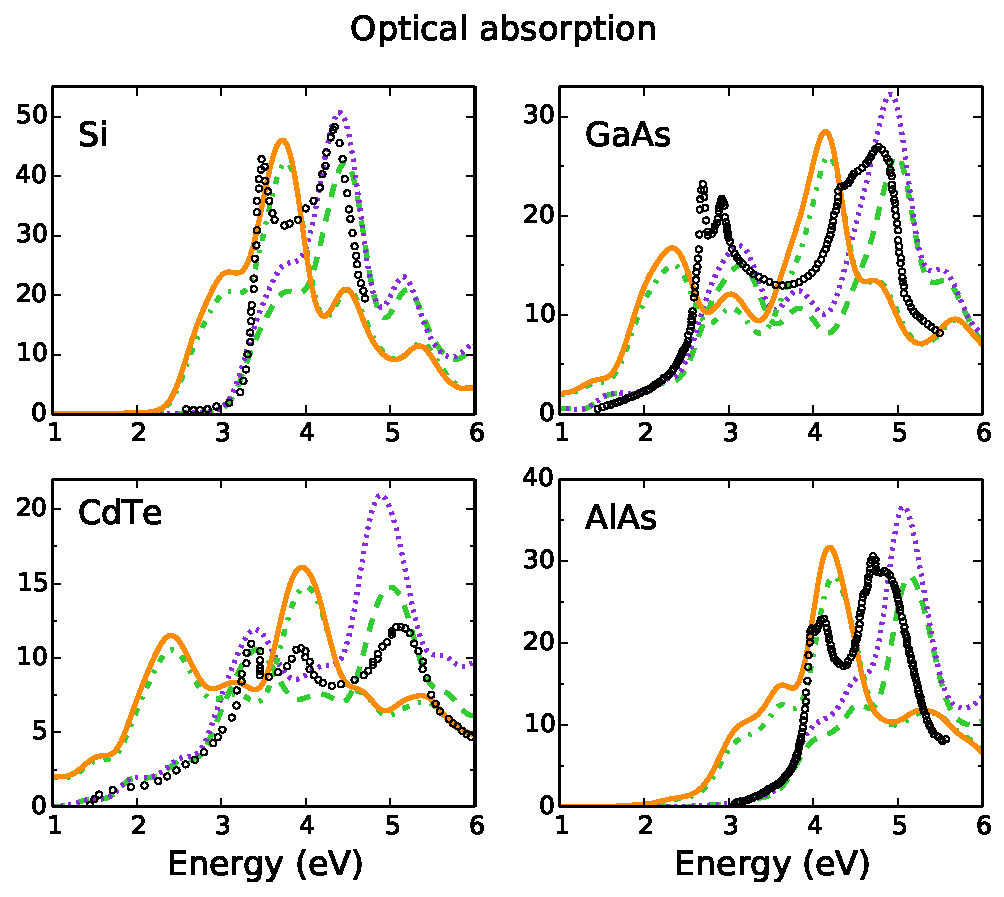
\includegraphics[width=0.7\textwidth]{Figures/Abs.pdf}
\caption{\footnotesize{Optical absorption in bulk Si (top left), GaAs (top right), CdTe (bottom left) and AlAs (bottom right): experimental optical absorption spectra (open circles) are compared with real-time simulations at different levels of approximation: TD-LDA (continuous orange line), RPA (green dash-dotted line), both without the scissor correction, and the IPA (violet dotted line) and RPA (green dashed line) with scissor correction.[Figure from Ref.~\cite{gruningtddf1}]}} \label{fg:epsblk}
\end{figure}


\subsection{Optical absorption}

The experimental optical spectra on Si~\cite{PhysRevB.36.4821}, GaAs~\cite{PhysRevB.35.9174}, CdTe~\cite{Adachi} and AlAs~\cite{GARRIGA} (Fig.~\ref{fg:epsblk}, black dashed lines) show qualitative similarities. They all present two main features, a peak at about 3-3.5 eV (referred as $E_1$) and stronger second peak at 4.5-5.0 eV (referred as $E_2$). In GaAs and CdTe, containing heavier third/fourth rows atoms, the $E_1$ peak is split because of the spin-orbit interaction.
Note that we do not include spin-orbit in the Kohn-Sham Hamiltonian and therefore we do not reproduce the splitting at any level of the theory. 

Figure~\ref{fg:epsblk} compares the experimental spectra with results obtained within the RPA and the TD-LDA (without scissor correction). For the considered systems the two approximations produce very similar spectra. As the only difference between the TD-LDA and the RPA is the microscopic xc potential, one can infer that the effect of the latter is minor as already discussed in the literature.~\cite{botti2007time,Onida} 
The most striking difference between the experimental and calculated spectra is the onset that is underestimated by 0.5--1.0~eV. When a scissor operator is added (see Ref~\cite{gruningtddf1}) the agreement is improved though for Si, GaAs and AlAs the $E_2$ peak is slightly blue-shifted and more importantly the $E_1$ peak is either underestimated or appears as a shoulder. Indeed the underestimation of the $E_1$ peak intensity in semiconductor by TD-LDA (and similar TD-DFT approximations) is well known and a signature of missing long-range correlation (see for example Refs.~\cite{PhysRevLett.43.387,PhysRevB.21.4656,botti2007time,Onida}). 
Comparison of the RPA spectra and the independent particle approximation (IPA) spectra shows that crystal local fields effects mostly reduces the intensity of the $E_2$ peak by 15--25\%.  
The experimental optical spectrum of CdTe is well caught within the RPA, but for the overestimation of the $E_2$ peak intensity.  

\begin{figure}[t]
\centering
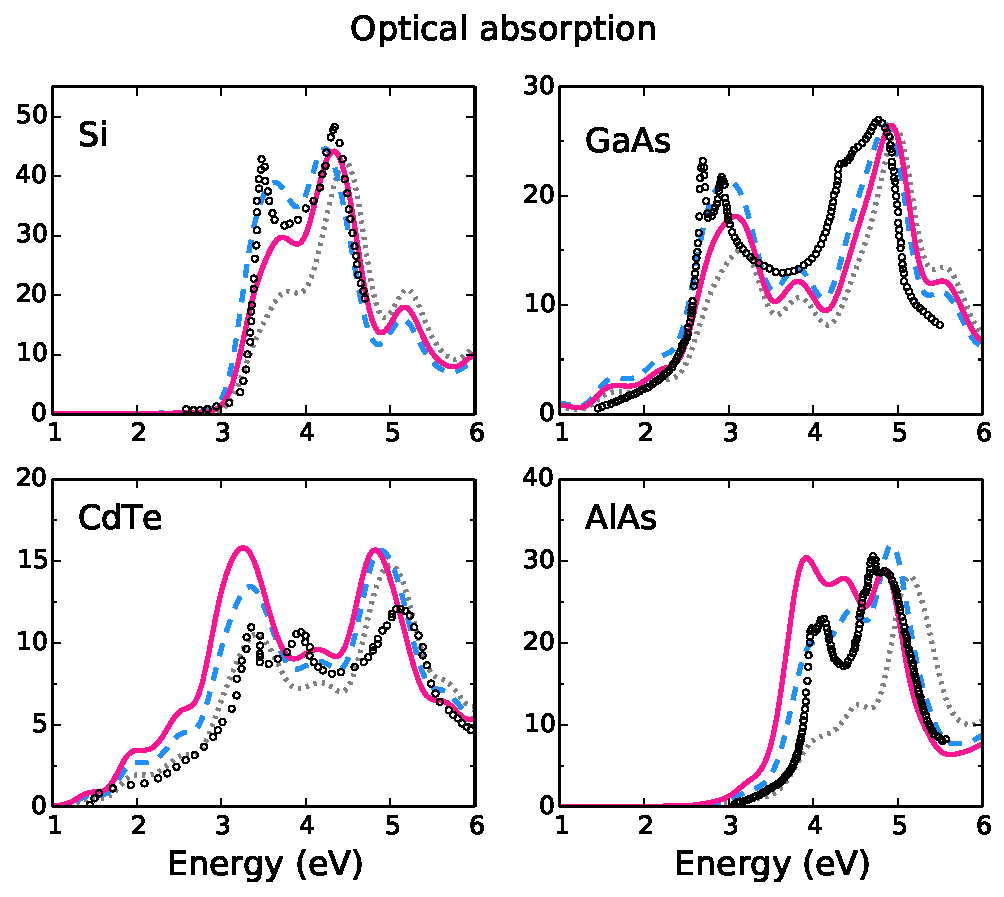
\includegraphics[width=0.7\textwidth]{Figures/Abs2.pdf}
\caption{\footnotesize{Optical absorption in bulk Si (top left), GaAs (top right), CdTe (bottom left) and AlAs (bottom right): experimental optical absorption spectra (open circles) are compared with real-time simulations at different levels of approximation: opt-PF (blue dashed line), JGM (pink continuous line), RPA(gray dotted line). All approximations include the scissor operator correction.[Figure from Ref.~\cite{gruningtddf1}] }} \label{fg:epsblk1}
\end{figure}


Figure~\ref{fg:epsblk1} shows the effects of the macroscopic xc field that is added through the approximated PFs discussed in Sec.~\ref{sc:ksef}. For Si, GaAs and AlAs a clear improvement is observed for the opt-PF: both intensity and position of the peaks are reproduced reasonably well. For CdTe adding the xc macroscopic field lead to an overestimation of the $E_1$ peak intensity which was well caught within the RPA. On the other hand the $E_1/E_2$ intensity ratio is better reproduce by the PFs than within RPA.
For the JGM-PF the agreement is in general less satisfactorily. In particular for Si the $E_1$ peak intensity is still visibly underestimated, while for AlAs it is overestimated. The main difference between the two approximation is the value of $\alpha$: in the opt-PF, $\alpha$ is a parameter optimised to reproduce the optical spectra; in the JGM-PF $\alpha$ is determined from the jellium with a gap model. The model does not reproduce the optimal value. For Si, $\alpha^{\sss JGM} \approx 0.11$ and for AlAs $\alpha^{\sss JGM} \approx 0.52$ respectively smaller and larger than the optimal value reported in Ref.~\cite{gruningtddf1}. It is worth to notice that the xc macroscopic field in the JGM-PF has as well a microscopic contribution. For AlAs this contribution is singled out in the right panel of Fig.~\ref{fg:effG} where it is shown to reduce slightly the absorption. For silicon (not shown) the microscopic contribution to the macroscopic field is negligible.

\subsection{SHG of GaAs, AlAs and CdTe} 



In zincblende structures the only independent non-zero SHG component~\cite{boyd} is $\chi^{(2)}_{xyz}$ (or its equivalent by permutation). The module of the calculated $\chi^{(2)}_{xyz}$ for the systems under study is reported in Fig.~\ref{fg:shg} and compared with experimental values where available.
Note that when the energies are not corrected by a scissor (left panel) for both GaAs and CdTe a large part of the energy range of the SH spectra is in the absorption region where both one-photon and two-photon resonances contribute to the intensity.  For AlAs the part of the SH spectra below 2~eV is instead in the transparency region of the material (only two-photon contributions).
When the scissor-correction to the energy is applied (right panel), the transparency region for GaAs and CdTe is below 1~eV and for CdTe below 3~eV. In the transparency region only two-photon resonances contribute. 
Comparing the TD-LDA with the RPA and the independent particle (IP)  spectra (left panel) shows that crystal local field effects (that tend to reduce the overall SH intensity) are partially compensated by the microscopic exchange-correlation effects (that tend to increase the SH intensity). In general both effects are relatively stronger than for the optical absorption. Applying the scissor correction does not correspond to a simple shift (like in the optical absorption case) but changes the spectra. Firstly the SH intensity is reduced overall (because of sum rules), secondly the intensity is redistributed as the scissor modifies the relative position of one-photon and two-photon resonances (that are shifted by a half of the scissor value). For GaAs and CdTe the addition of macroscopic correlation through the approximated PF leads to an enhancement of about 40\% in GaAs and 80\% in CdTe with respect to the RPA. On the other hand as discussed for those systems local field effects are very large and in fact the spectra form the PF are not significantly different than at the IP level, meaning an almost exact cancellation of the crystal local effects and the macroscopic xc effects as describe by the approximated PFs. Only in the case of AlAs, the macroscopic correlation enhances significantly the SH, adds features and redistributes relative weights with respect to the IPA. 
Regarding the comparison with experiment (right panel), in GaAs the peak at 1.5~eV and the feature at 2.2~eV in the experimental SHG are fairly reproduced by the opt-PF and  JGM-PF approximations. All approximations significantly overestimate the SH for energies below 1~eV. A similar breakdown of the opt-PF approximation (that within the response theory context corresponds with the long-range corrected kernel) has been observed by Luppi and coworkers and traced back to the errors in the theoretical macroscopic dielectric function.~\cite{PhysRevB.82.235201} For CdTe, the approximation that is closer to experimental results (which however are available only around 1~eV) is the RPA while both PF approximations overestimate the experimental SH. This is consistent with the results for optical absorption for which the RPA gives the best agreement among all approximations considered.
\begin{figure}[H]
\centering  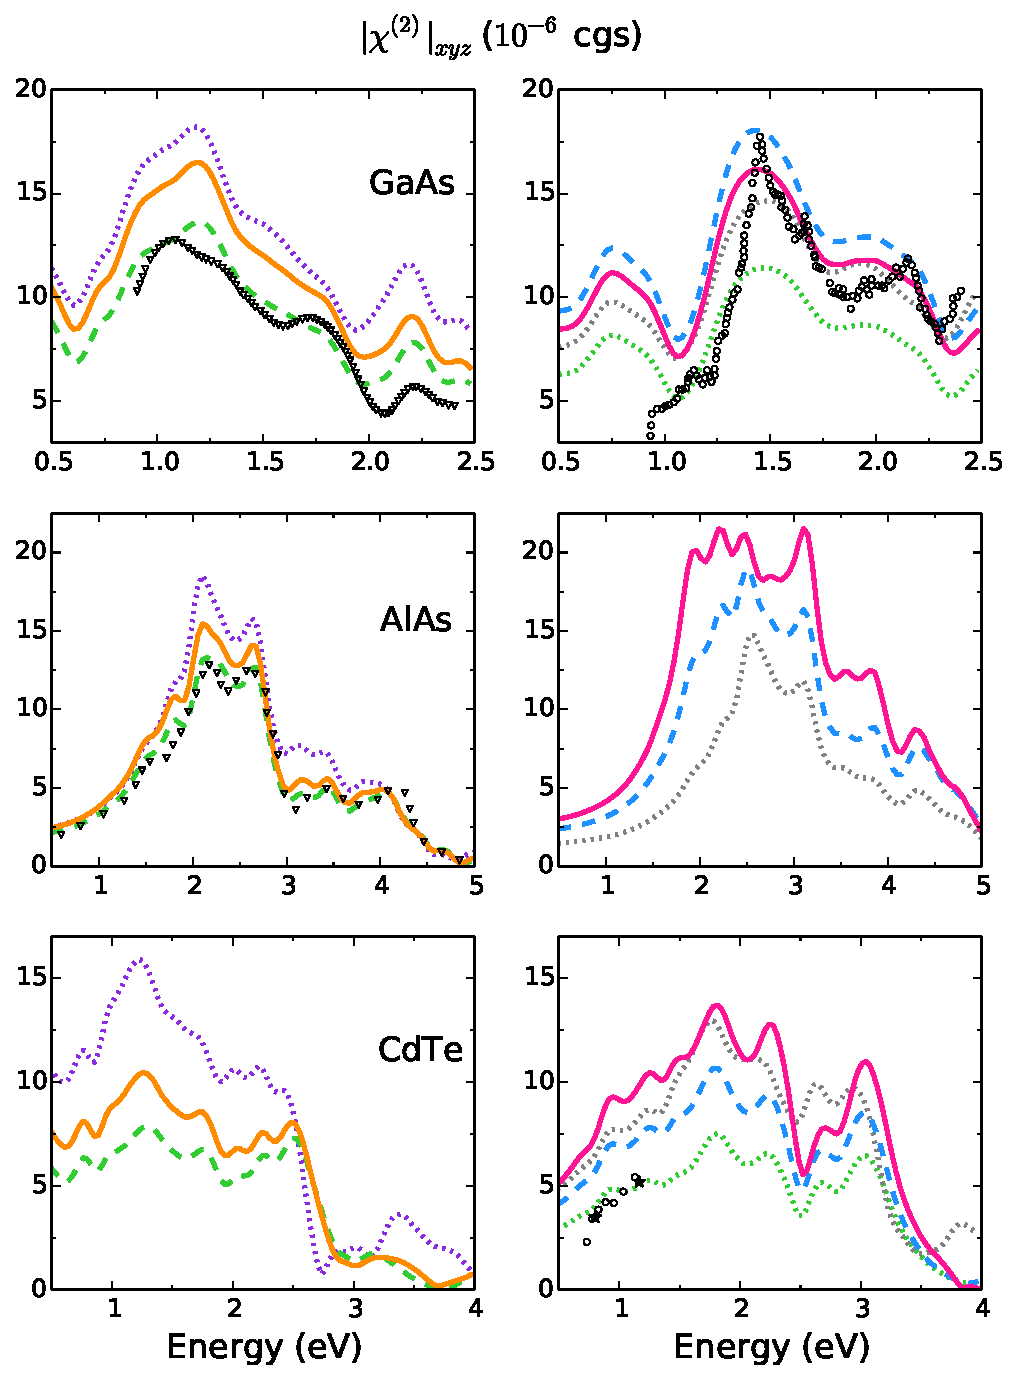
\includegraphics[width=0.8\textwidth]{Figures/SHG.pdf}
\caption{\footnotesize{SHG spectra of GaAs (top panels),  AlAs (middle panels) and CdTe (bottom panels) obtained from real-time simulations at different levels of approximation. Left panels: IPA (dotted violet), RPA (dashed green) and TD-LDA (continuous orange)---all without scissor operator correction. For comparison we included the RPA spectrum of GaAs and AlAs calculated by Luppi et al.\cite{PhysRevB.82.235201} (open triangles) \label{fg:shgblk}. Right panels: opt-PF (dashed blue) and JGM-PF (continuous pink) are compared with IPA (dotted gray) and RPA for CdTe and GaAs (dotted green). Available experimental results are shown for GaAs (open circles)~\cite{bergfeld2003second} and CdTe (open circles~\cite{Shoji:97} and stars~\cite{Jang:13}).\label{fg:shg} [Figure from Ref.\cite{gruningtddf1}] }}
\end{figure}

We have also compared our results from real-time simulations with those obtained from a response approach by Luppi and co-workers~\cite{PhysRevB.82.235201} and we found a good agreement, slightly better than our previous work\cite{nloptics2013} thanks to the higher order approximation for the covariant derivative [Eq.~\eqref{eq:wkhat2}]. In the left panel of Fig.~\ref{fg:shg} we show for example the comparison for the RPA. There is a very good correspondence between the two spectra for AlAs. For GaAs there are small, but still visible differences which we argue are due to the different pseudopotentials used. In fact we obtain a similar variation in our results when repeating the calculations with different pseudopotentials. It is known that SHG is very sensitive to changes in the electronic structure and that is turn changes when using different pseudopotentials. This is particularly true in the case of GaAs and the sensitivity on the pseudopotential choice was also observed in the referenced calculations.  
Note that in the pseudopotentials we used $d$ orbitals are considered as core electrons, whereas they are included as valence electrons in the calculation of Luppi and coworkers.~\cite{PhysRevB.82.235201} On the other hand pseudopotentials including $d$ electrons that we were testing did not provide a much better agreement.  

\subsection{THG of Si} 



Figure~\ref{fg:siX3ab} shows the calculations for $A=|\chi^{(3)}_{1111}|$ and $B=|3\chi^{(3)}_{1212}|$, the modules of the $1111$ and $1212$ components of the THG of Si~\cite{Moss:89}. These were deduced from calculations with the input field either along the $x$ or along the $xy$ direction.

The TD-LDA spectra (top panels) both present two main features, a peak around 0.9~eV (three-photon resonance with $E_1$) and a shoulder around 1.4  eV (three-photon resonance with $E_2$). Both features are more intense and pronounced in the $|3\chi^{(3)}_{1212}|$. Results within TD-LDA resemble closely those obtained within the RPA and IP approximation. For the $E_1$ three-photon resonance the microscopic exchange-correlation effects cancel with the local-field effects, so that TD-LDA almost coincides with the IP approximation. For higher energies instead, the TD-LDA and RPA spectra are practically identical. Applying a scissor operator does not simply shift the peaks by an amount of about 1/3 of the scissor value. The overall intensity of the spectra is reduced (as expect from sum rules) and as well the relative intensity of the $E_1$/$E_2$ resonances changes. Specifically the ratio is close to or even smaller than $1$ in the scissor corrected spectra, while is $\approx 1.2-1.3$ in the uncorrected spectra. The macroscopic exchange-correlation introduced with the approximations for the PF (bottom panels) enhances the intensity of the spectra and as well the $E_1$/$E_2$ ratio. Consistently with what observed for the linear response, the largest $\alpha$ (opt-PF for silicon) produces the largest correction.

\begin{figure}[ht]
\centering
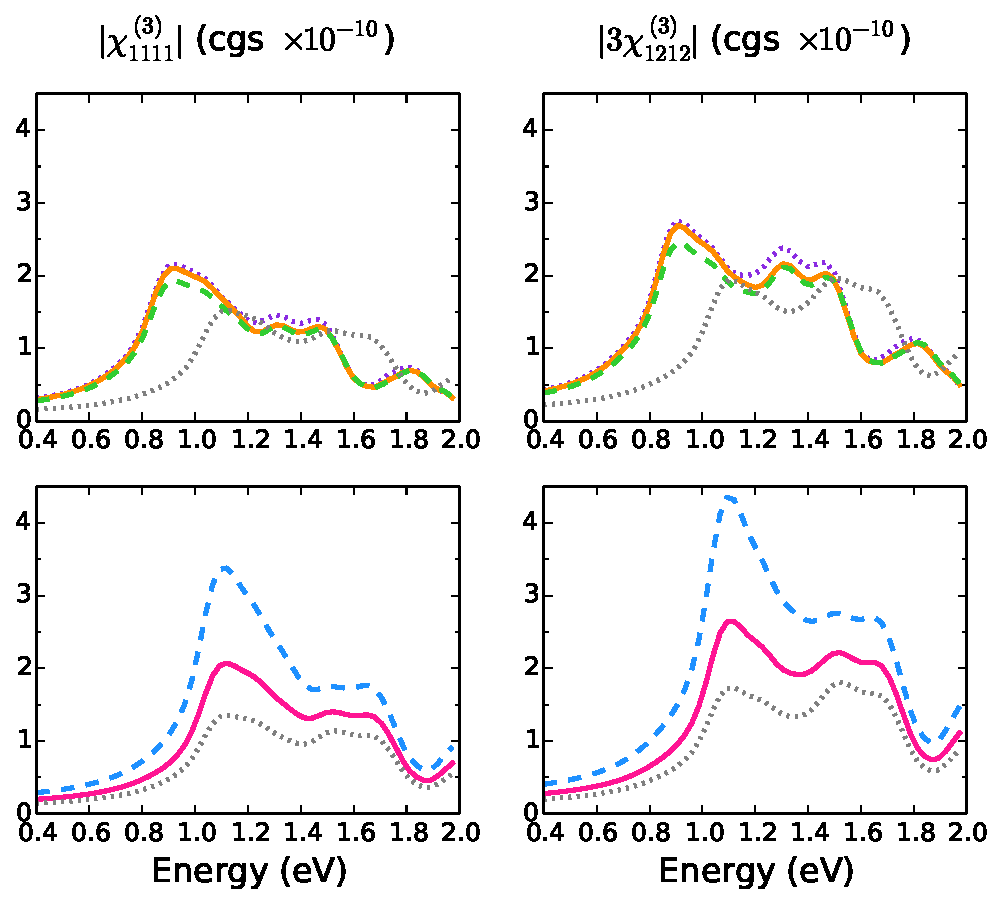
\includegraphics[width=0.9\textwidth]{Figures/X3.pdf}
\caption{\footnotesize{THG of Si: $|\chi^{(3)}_{1111}|$ and $|3\chi^{(3)}_{1212}|$ components (see text). Spectra obtained from real-time simulations at different levels of approximation. Top panels: TD-LDA (continuous orange line), RPA (green dashed line), IPA (dotted violet line) without scissor operator correction are compared with and IPA (gray dotted line) with scissor operator correction. Bottom panels: JGM-PF (continuous pink line), opt-PF (blue dashed line) and RPA (gray dotted line) with scissor operator correction. [Figure from Ref.\cite{gruningtddf1}] }} \label{fg:siX3ab}
\end{figure}
Experimental measurements are available for the ratio $R_1$ between the THG signal obtained with $45$ and $0$ incident angles and for the ratio $R_2$ between the THG signal obtained with circularly polarised light and linearly polarised light at $0$ incident angle. From those measurements then $\sigma = |1 - B/A|$ and the phase $\phi(B/A)$ can be deduced.~\cite{Moss:89} The experimental results are reported in Fig.~\ref{fg:siX3an}. Both $\sigma$ and $\phi(A/B)$ present two features at about 1.1~eV and 1.4~eV in correspondence of the three-photon $E_1$ and $E_2$ resonances. All the theoretical results are very similar irrespective of the approximation used and the differences observed for the $A=|\chi^{(3)}_{1111}|$ and $B=|3\chi^{(3)}_{1212}|$ in Fig.~\ref{fg:siX3ab}. The results from the scissor corrected approximations (right panels) are just shifted by 1/3 of the scissor operator. When compared with the experiment all the approximation reasonably reproduce the behaviour at energies lower than 1~eV. However for both $\sigma$ and $\phi(A/B)$ (we consider here only the scissor corrected approximations which have resonances at the correct energies) the peak in correspondence of the $E_1$ resonance is missing and the feature in correspondence of the $E_2$ resonance much less pronounced than in experiment. When compared with calculations from Moss and coworkers~\cite{Moss1990} at the independent particle level from the electronic structure calculated either with empirical tight-binding and semi-ab-initio band-structure techniques, the intensity we found for $A$ and $B$ are similar to the latter, but the main spectral features are similar to the former. To notice that the THG based on empirical tight-binding shows in the $\sigma$ and $\phi$ spectra a peak at 1.1~eV.    

\begin{figure}[hb]
\centering
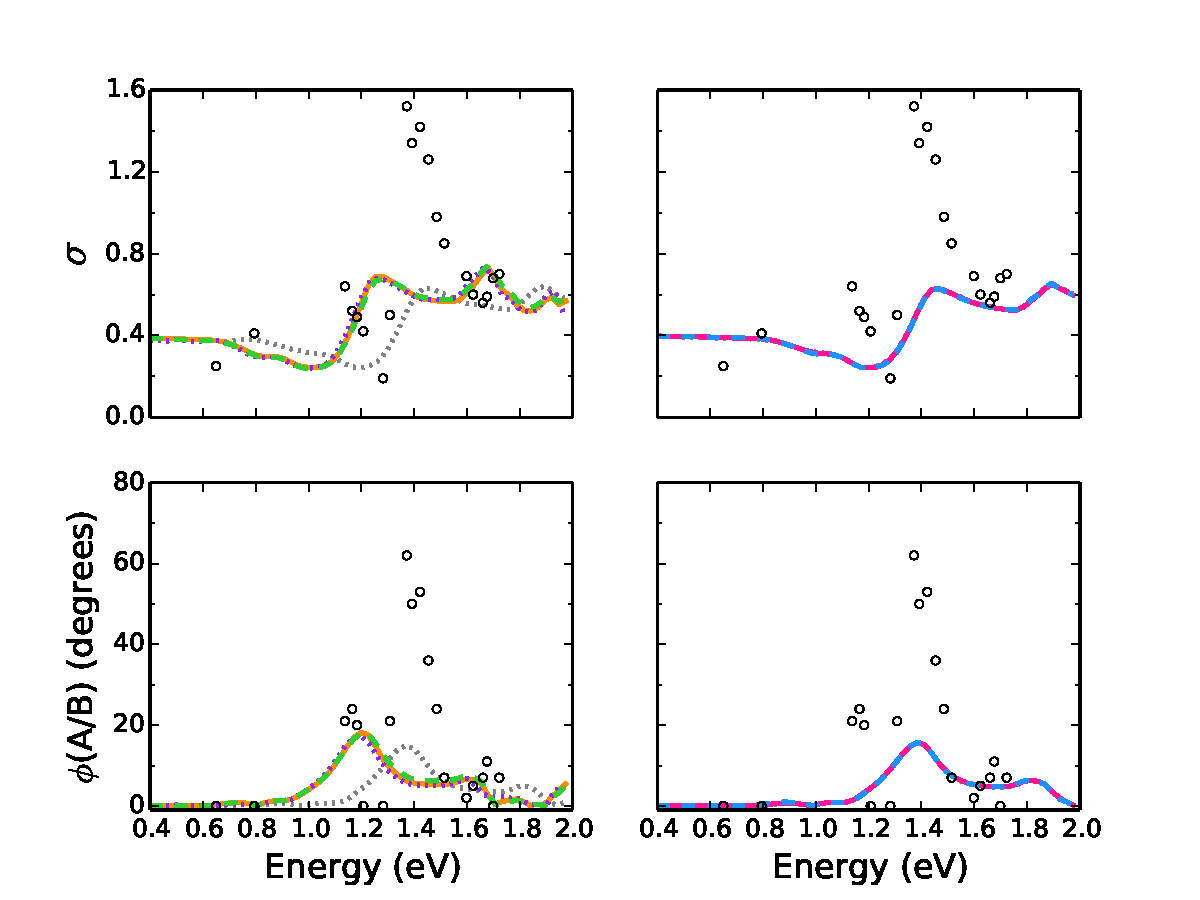
\includegraphics[width=1\textwidth]{Figures/anysX3.pdf}
\caption{\footnotesize{THG of Si: anisotropy parameters $\sigma$ and $\phi$ (see text). Experimental data (open circles)\cite{Moss:89} compared with results obtained from real-time simulations at different levels of approximation. Left panels: TD-LDA (continuous orange line), RPA (green dashed line), IPA (dotted violet line) without scissor operator correction are compared with the IPA (gray dotted line) with scissor operator correction. Right panels: JGM-PF (continuous pink line), opt-PF (blue dashed line) and RPA (gray dotted line) with scissor operator correction.[Figure from Ref.\cite{gruningtddf1}] }} \label{fg:siX3an}
\end{figure}

%%%%%%%%%%%%%%%%%%%%%%%%%%%%%%%%%%%%%%%%%%%%%%%%%%%%%%%%%%%%%%%
\section{Discussion}

It is interesting to analyse how an apparently simple approximation such as $\alpha \PP$ correctly ``distinguishes'' where to increase the optical absorption spectrum at RPA level. This information is ``encoded'' in the macroscopic polarisation. In fact, in the linear response limit the effective Kohn-Sham electric field within the proposed PF approximations takes the form $$\Efield^{s} (\omega)= [1 -\alpha \chi(\omega)] \Efield^{\text{tot}} (\omega).$$ That is, the intensity of the applied field is either amplified or reduced depending on the sign of $\text{Re}\chi(\omega)$---as $\text{Im}\chi(\omega) \ge 0$ for any positive $\omega$. In Fig.~\ref{fg:epsanl} (upper panel) we see that indeed the sign of $-\text{Re}(\chi_0)$ follows closely that of the correction induced by $-\alpha P$. 
To gain an insight on how the sign of $\text{Re}(\chi_0)$ is linked to the localisation of the excitation we consider the phasor representation of $\chi_0(\omega) = |\chi_0(\omega)|\exp{(i\phi)}$: the complex argument $\phi$ (see bottom panel of Fig.~\ref{fg:epsanl}) gives the phase delay between $\PP$ and $\Efield$. In particular a delay of $\phi = \pi/2$ corresponds to in-phase oscillation of the macroscopic polarisation current $\JJ$ ($-\partial \PP/\partial t$) with $\Efield$: where the optical absorption is negligible those oscillations are plasmons; in regions with non-negligible optical absorption they can be considered as a signature of delocalized excitations (note that in fact the optical absorption it as a maximum at $\phi=\pi/2$).  Heuristically, for more localized excitations we may expect a phase delay larger than $\pi/2$, and for delocalized excitations a phase delay smaller than $\pi/2$.
Then, the $\cos\phi$, and $\text{Re}(\chi)$ which is proportional to it, are negative for localized excitations and positive for the more delocalized ones. A correction proportional to  $-\text{Re}(\chi)$ then increases the absorption in correspondence of more localised excitation and decreases it for more delocalized excitations. Note as well that in the RPA the phase delay is overestimated. Then the absorption, proportional to $\sin\phi$ is too small for $\phi > \pi/2$ (localized excitation) and too large for $\phi < \pi/2$ (delocalised  excitation).
\begin{figure}[ht]
\centering
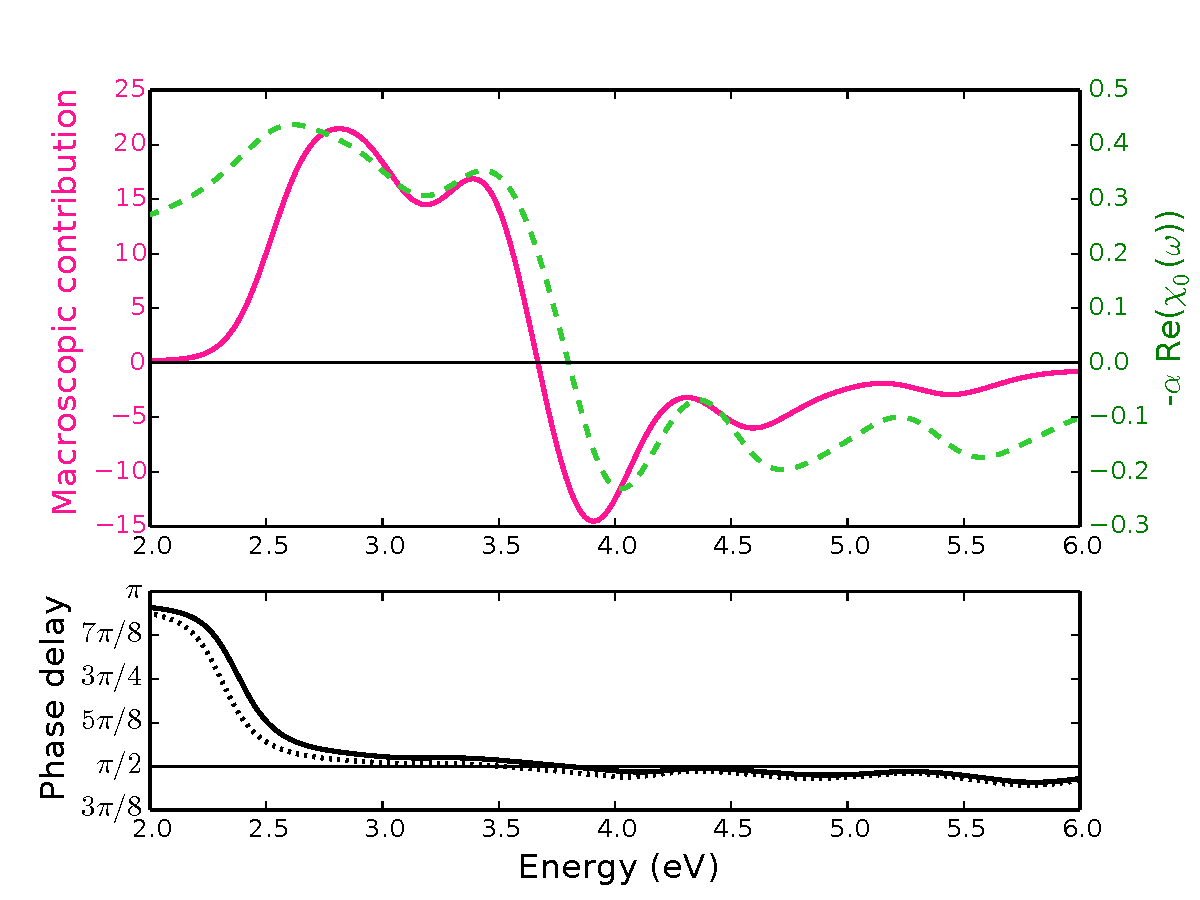
\includegraphics[width=0.6\textwidth]{Figures/Analysis.pdf}
\caption{\footnotesize{Upper panel: Macroscopic contribution to the optical spectrum of Si calculated as the difference between the the opt-PF  and the RPA optical absorption spectra (pink continuous line) compared with $-\alpha \text{Re}(\chi_0)$ (green dashed line). Bottom panel: phase delay $\phi$ between the polarisation and the applied electric field as a function of the applied field frequency at the RPA (dotted line) and opt-PF (continuous line) level of approximation. The horizontal line highlight the $\phi =\pi/2$ delay. See text.[Figure from Ref.\cite{gruningtddf1}] }} \label{fg:epsanl}
\end{figure}


\section{Summary and conclusions}
We have implemented a real-time density functional approach suitable for infinite periodic crystals in which we work within the so-called length gauge and calculate the polarisation as a dynamical Berry phase.~\cite{souza_prb}        
This approach, in addition to the electron density considers also the macroscopic polarisation as a main variable and extends to the time-dependent case the DPFT introduced in the nineties~\cite{Gonze1995,Resta1996,Vanderbilt1997,Martin1997} to correctly treat IPC in electric fields within a density functional framework. In the corresponding time-dependent KS equations next to the microscopic xc potential also appears a macroscopic xc electric field which is a functional of the macroscopic polarisation (and eventually of the microscopic density).
We have derived approximations for the xc electric field exploiting the connection with long-range corrected approximations for xc kernel within the linear response theory. We have considered two approximations, the optimal polarisation functional, linked to the  long-range corrected xc kernel proposed on Ref.~\cite{LRC} and the Jellium with a gap model polarisation functional linked to the analogous approximation for the xc kernel.\cite{jgm}
We have applied this approach, that we refer to as real-time DPFT, to calculate the optical absorption, second and third harmonic generation in different semiconductors (Si, GaAs, AlAs and CdTe). We have compared results with ``standard'' real-time TD-DFT, namely without macroscopic xc effects, and to experimental results where available. The general trend is an overall improvement over standard TD-DFT as to be expected from the results obtained within the response framework.~\cite{LRC} Of the considered approximations, the opt-PF provides the best agreement with the experiment.
We verified this finding also with other materials, the zinc chalcogenides ZnX (X= S, Se, and Te)\cite{gruningtddf2}, not reported in the present chapter.

The approach here proposed combines the flexibility of a real-time approach, with the efficiency of DPFT in capturing long-range correlation. It allows calculations beyond the linear regime (e.g. second- and third-harmonic generation, four-wave mixing, Fourier spectroscopy or pump-probe experiments) that includes excitonic effects. It is an alternative approach to real-time TD-DFT for extended system proposed by Bertsch, Rubio and Yabana.\cite{PhysRevB.62.7998} At difference with our approach the latter uses the velocity gauge---which has the advantage of using the velocity operator that is well defined in periodic systems---rather than the position operator that requires special attention. On the other hand,  although this approach have shown promising results,\cite{PhysRevB.85.045134,goncharov2013nonlinear} it turns to be quite cumbersome for studying response functions beyond the linear regime due to the presence of divergences that in principle should cancel, but that are difficult to treat numerically.\cite{PhysRevB.52.14636} Furthermore non-local operators---such as pseudo-potentials or the scissor operator---are cumbersome to threat in velocity gauge\cite{tokman} while they are trivial in length-gauge.
\begin{figure}[ht]
\centering
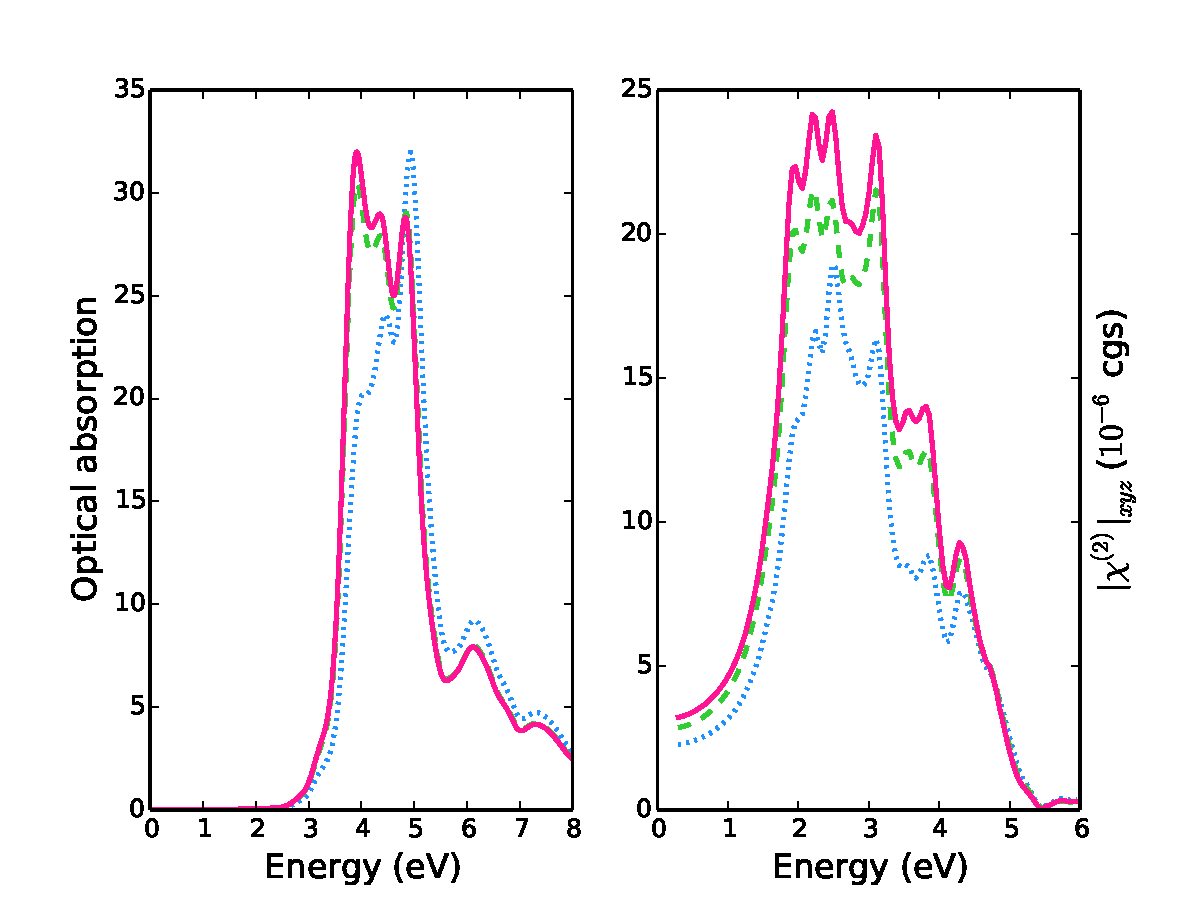
\includegraphics[width=0.6\textwidth]{Figures/Geff.pdf}
\caption{\footnotesize{Effect of microscopic components in the JGM-PF on the optical absorption (right panel) and SHG (left panel) of AlAs. The plots compare JGM-PF spectra with (green dashed line) and without microscopic effects (magenta continuous line) and the opt-PF (blue dotted line). [Figure from Ref.\cite{gruningtddf1}] }}
%kin the Brillouin zone
\label{fg:effG}
\end{figure}

Similarly to any density-functional approaches, a delicate point is the approximation of the xc effects. In addition to the xc potential as in standard DFT, in this approach we also need an approximation for the macroscopic xc field. Though for the systems here studied the opt-PF approximation seems to work well, such a good performance cannot be expected in general. For example, based on the experience from linear response calculations, this approximation is not expect to work very well for large gap insulators or systems with a reduced dimensionality (e.g. nanostructures or layers) in which the electronic screening is small.~\cite{PhysRevB.68.205112} Furthermore, in the opt-PF the $\alpha$ is chosen has a material dependent parameter rather than obtained from first-principles. In this respect within the other approximation here studied, JGM-PF, $\alpha$ is determined from first-principles but not always has the optimal value. Further studies then should try to develop universal approximations to the polarisation functional, possibly going beyond the linear response formulation that was here used in the derivation of the polarisation functionals.  
